\chapter{Experimental}

This chapter describes the apparatus at Colorado State University, which has been used for all described studies of Ba/Ba\textsuperscript{+} fluorescence in SXe after deposition in vacuum.  Our main barium source, the Ba\textsuperscript{+} ion beam, is first described, as well as a purely Ba neutral source.  The co-deposit of Ba/Ba\textsuperscript{+} with Xe gas onto a cold sapphire window, subsequent laser excitation, and finally the collection optics for the fluorescence are described.

\section{Ion Beam}

The full ion beam is shown in Fig. \ref{fig:ionbeam}.  This is a clean source of Ba\textsuperscript{+} which can do a very wide range of deposit sizes, from billions of ions in a focused laser region all the way down to the single-ion level {\color{gray}, and even deposits sparse enough to scan a laser over spatially separated ions (may only want to say that if we have those scans)}.

\begin{figure} %[H]
        \centering
                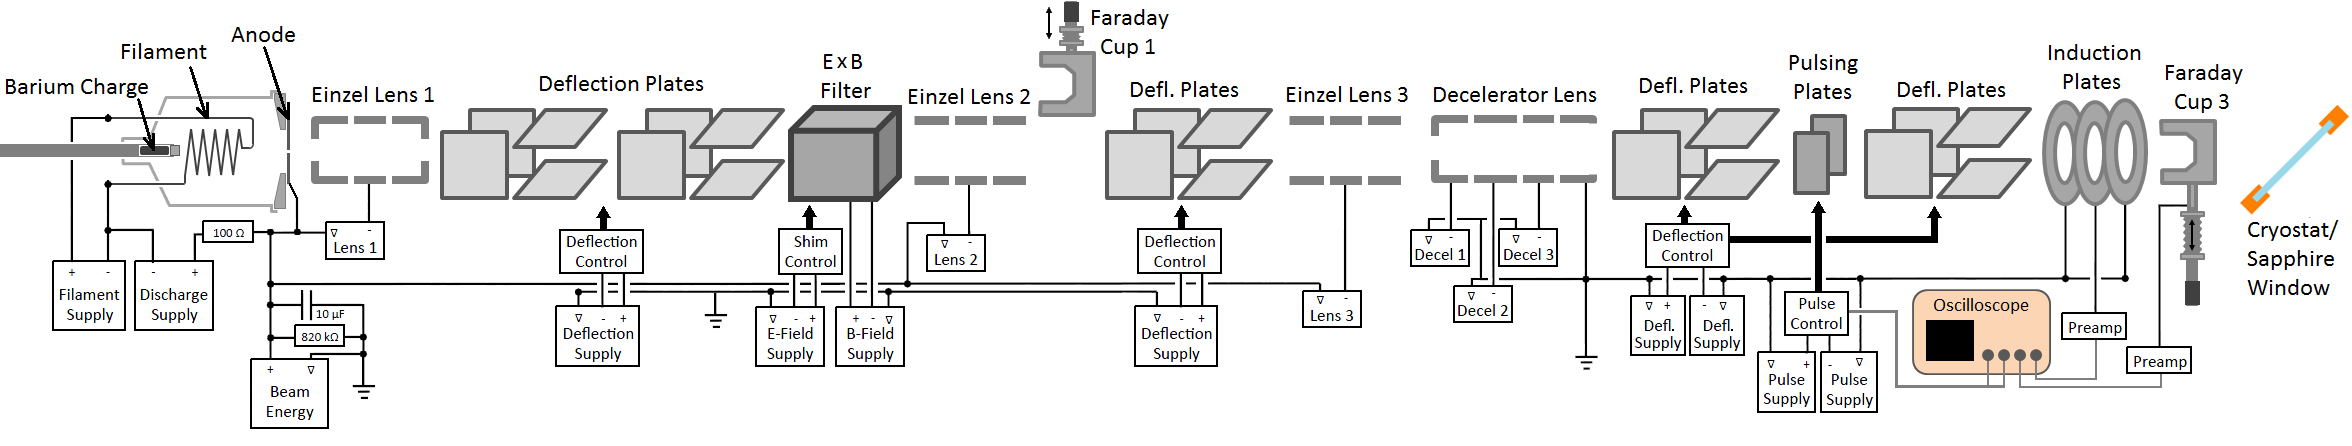
\includegraphics[angle=90,width=.25\textwidth]{figures/ionBeam.png}
                \caption{Ba\textsuperscript{+} ion beam.}
\label{fig:ionbeam}
\end{figure}

\subsection{Ion Source/Acceleration}

Ba\textsuperscript{+} ions are produced in a Colutron ion gun system \cite{Colutron}.  The source is shown in Fig. \ref{fig:ionsource}.  A solid barium charge is placed into the hollowed end of a stainless steel rod, which is then inserted into the discharge chamber, near the hot filament.  The barium vaporizes, and escapes the hollowed rod around a loosely threaded set screw.  The source is designed to produce a discharge between the anode plate and the filament cathode, through an argon buffer gas leaked into the source chamber.  This controlled discharge would then also ionize atoms, vaporized  from the solid charge, to produce the desired ion beam, and Ar ions would be filtered out.  However, to avoid contamination of the solid matrix with residual Ar gas, the buffer gas is not used in this work.  We are still able to maintain a discharge between the filament and anode circuits.  The longevity of our ion current from a single charge (at least several 10s of hours) suggests that Ba is coating the inner walls of the chamber and is depleted slowly.  This is supported by the observation of white oxidation of the inner source parts after a few minutes of exposure to air when opening the system.  The discharge produces a plasma, containing barium ions, which escapes the chamber through a small hole in the anode, where it enters the acceleration potential.  The acceleration potential is 2~kV, between the ion source anode and an aperture, which is the first element of the Einzel lens 1.  This lens approximately collimates the ion beam for passage through the E$\times$B velocity filter.

\begin{figure} %[H]
        \centering
                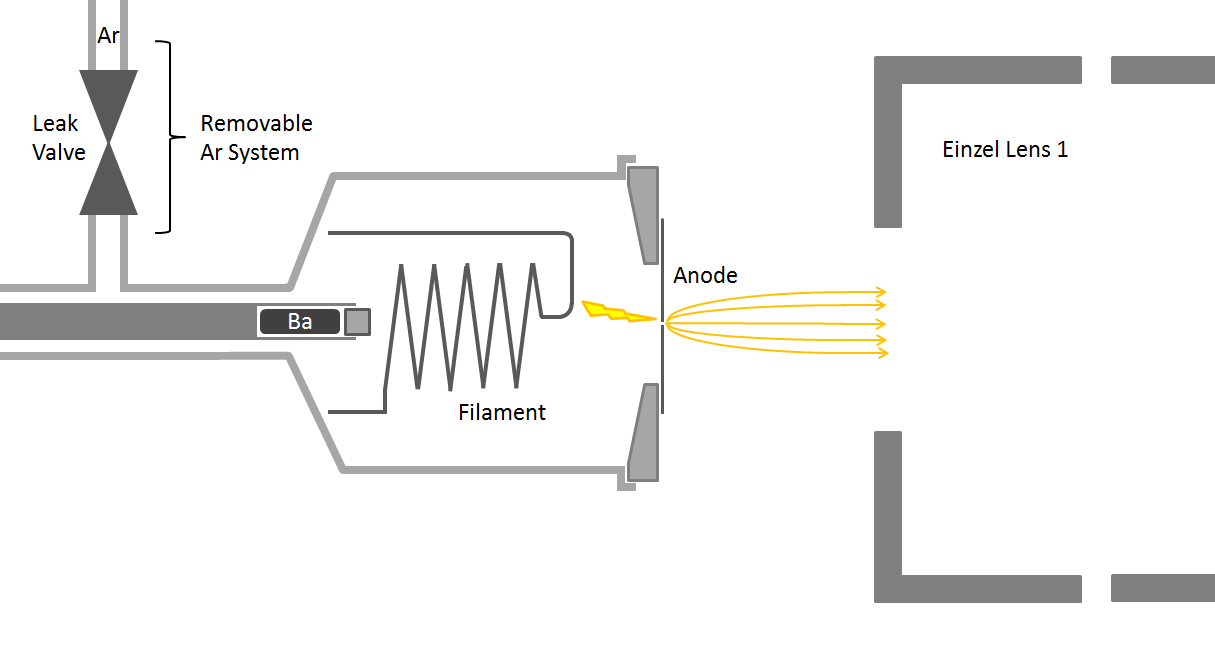
\includegraphics[width=.95\textwidth]{figures/ionSource.png}
                \caption{Ba\textsuperscript{+}/Ar\textsuperscript{+} ion source.}
\label{fig:ionsource}
\end{figure}

\subsection{E$\times$B Velocity Filter}

The E$\times$B velocity filter selects Ba\textsuperscript{+} by creating perpendicular electric and magnetic fields, which produce opposing forces on charged particles moving straight through the filter.  The opposing forces will be equal for ions with velocity $v = \frac{E}{B}$.  Since ion velocity is determined by mass ($m$), charge ($q$) and beam potential ($V$), the filter selects ions satisfying Eq. \ref{eqn:massfilt}:

\begin{equation}
\frac{m}{q} = \frac{2 V B^{2}}{E^{2}}
\label{eqn:massfilt}
\end{equation}

\noindent
where $B$ and $E$ are the magnetic and electric fields, respectively.  Those fields are chosen such that the forces are equal for Ba\textsuperscript{+}.  Other ions will be deflected.  

The E$\times$B filter is shown in Fig. \ref{fig:exb}.  Electromagnets provide the vertical magnetic field.  Electrode plates and field-shaping guard rings provide the horizontal electric field.  The guard rings prevent a lensing and astigmatism effect from fringe fields of the plates \cite{Colutron}.

\begin{figure}[h]
        \centering
                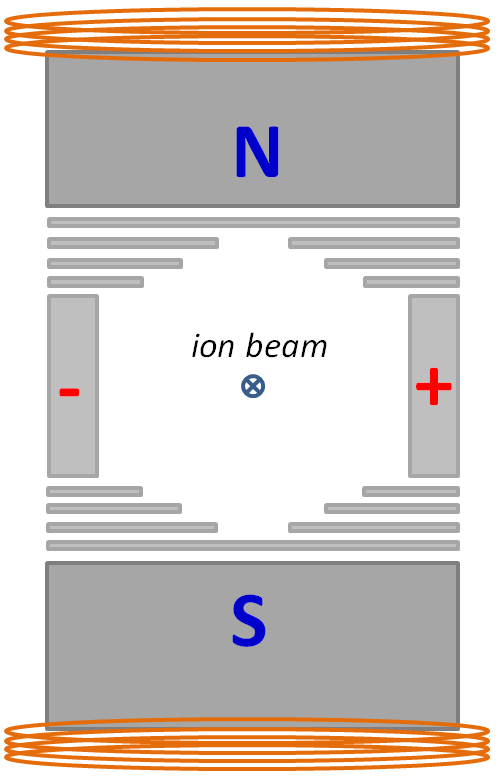
\includegraphics[width=.7\textwidth]{figures/ExB.png}
                \caption{Colutron E$\times$B ion velocity filter.}
\label{fig:exb}
\end{figure}

\emph{\color{gray}If we need mass scans, we probably need to do new ones with a constant magnetic field, and Ar\textsuperscript{+} and Ba\textsuperscript{+} in same day.  Past scans were all over the place, partly because we were changing beam settings, but new peaks are not very consistent either.}
%To determine the mass components of the beam, the electric field can be scanned.  Mass scans of the Ba\textsuperscript{+} beam is shown in Fig. [ref mass scan fig], as well as of an Ar\textsuperscript{+} beam.  The known mass of Ar aids in calibrating the magnetic field, which differs from the calculation given by Colutron, likely due to hysteresis in the magnet.  \emph{\color{gray}The Ba\textsuperscript{+} peak agrees with the Ba mas s... }

\subsection{Other Beam Components}

The first three sets of deflection plates can be used for beam diagnostics, and are set to 0~V during normal operation.  The deflection plates just before the pulsing plates, H1 and V1, are set to constant values of 50~V and 0~V, respectively, which have been selected such that the beam, in both pulsing and continuous modes, can be deposited at the sapphire window for reasonable settings on the final deflection plates, H2 and V2.  As described in \ref{subsec:ionDepCal}, different settings in H2/V2 are required for peak ion current in cup 3 vs. peak deposit at the window.

Einzel lens 2 focuses the beam the pass through the aperture in the first element of the decelerator lens.  Einzel lens 3 is not used in this setup.  The decelerator lens can be used to vary Ba\textsuperscript{+} deposit energy, but it in this work it acts as an Einzel lens with only the second element at voltage, and it focuses the beam at Faraday cup 3 (there is no Faraday cup 2 in this setup).  Faraday cup 3 measures the ion current during experiments, and is retracted when deposits are being made.  Its use in deposit calibration is described in \ref{subsec:ionDepCal}.  Faraday cup 1 is used for beam diagnostics, and is usually retracted on its bellows.  

\subsection{Ion Beam Pulsing}

When running in pulsing mode, the pulsing plates are first set to 200~V and -200~V to deflect the beam, and are pulsed to 0~V for 1~$\mu$s for each pulse.  The pulsing circuit is shown in Fig. [ref fig pulsing circuit, \textbf{ref Shon thesis if this is same figure}].  Square waves, triggered by LabVIEW at 500~Hz, enter the circuit at [x]. {\color{red}[describe how the pulse happens]}

The induction plates observe pulses during a deposit.  Pulses just prior to a deposit can be observed by cup 3 as well as the induction plates, for a local measurement of ion current in the pulses.  eV Products pre-amplifiers convert the ... [put this before scope picture?] [have a figure of the shaped plots too].  An example of an oscilloscope readout of {\color{red}16} averaged pulses is shown in Fig. [ref fig scope pulse -- in caption, explain v-divided plate signals].  [make this with the 8-7 Ba+]

Pulsing data also provides confirmation that the beam is composed of Ba\textsuperscript{+}.  The time between the center of the pulsing plate voltage overlap and the center of the pulse measured by the Faraday cup, along with a measurement of the distance traveled, provides a velocity measurement of the ions.  This distance of 31.5~cm $\pm$ 1.0~cm, \emph{\color{red}check the d measurenet -- can you make the uncertainty +- .5 cm?  and look at older Ar+ ones  for consistency because 6-25 gives like 35.7 +- 5}

\subsection{Calibration of Ion Deposit}
\label{subsec:ionDepCal}

To calibrate the signal at cup 3 to an ion density at the sapphire window, another Faraday cup (cup w) is attached to the cold finger in place of the sapphire window.  Firstly, the ratio in $\frac{fC}{pulse}$ between cup 3 and cup w is measured ($\equiv f$).  Then, knowing the radius of cup w lets one determine the ion density per pulse at the sapphire window:

\begin{equation}
\frac{ions}{pulse \times m^{2}} = \frac{C f}{A e}
\label{eqn:ion_density}
\end{equation}

\noindent
where $C$ is $\frac{fC}{pulse}$ at cup 3, $A$ is the area of cup w, and $e$ is the elementary charge.  The required settings of the final deflection plates H2 and V2 are also determined by cup w.  These typically differ from the peak values for cup 3 by about ???, corresponding to ??? mm.

{\color{gray}\emph{Talk about beam size?}}

\section{Ba Getter Source}

BaAl$_{4}$ getters are neutral Ba sources typically used to grab reactive gas molecules in purifiers and vacuum tubes.  \emph{\color{red}don't say we, and look up how they work ... is it a rxn even in the non-Ni-powder case (our wire)?}We can use a getter as a source of neutral Ba.  It is very helpful to have a completely different Ba source, especially a neutral-only source, in identifying observed fluorescence peaks.  This is discussed further in \ref{subsec:peakIdentify}.

The getter used briefly in this work is an endothermic ... getter wire ... {\color{gray}[describe it]} ... show diagram, maybe also of it in the system at same position as cup 3.

\section{Sample Deposition}

The Ba\textsuperscript{+}/Ba are co-deposited with Xe gas onto a cold sapphire window tiled at 45$^{\circ}$.  Sapphire has good thermal conductivity at low temperature and good optical transparency in the visible.  Xe freezes around {\color{red}73~K} in vacuum.  The window is held to a cold finger (Fig. 6x, picture of), cooled by a -brand- cryostat. % -brand- said {\color{red}brand}, but that had errors

Before barium ions are let through, xenon gas is allowed to flow, controlled by a leak valve, onto the cold sapphire window, where it freezes and begins growing the solid matrix.  The Faraday cup is then retracted, to clear the path for barium ions.  The cup serves as a shutter for DC deposition, or if pulsing is being used, they are performed at this time.  Barium ions land in the solid xenon as the matrix continues to grow.  The cup is then replaced, and the xenon leak stopped.

[show new fringe tests]

\subsection{Laser Excitation}

um

[astigmatism in window, and data for that with compensator]

[also could put in the astigmatism check on the laser itself (consistent w/ zero) (pg. 24 of Chris's book)]

[waist measurements -- apply calibration uncertainty to the good motor-stage ones]

\subsection{Collection Optics}

talk about all that, including spectrometer